\documentclass{beamer}

\usepackage[utf8]{inputenc}
\usepackage[T1]{fontenc}
\usepackage{graphicx}
\usepackage{listings}
\usepackage{xcolor}

\definecolor{codegreen}{rgb}{0,0.6,0}
\definecolor{codegray}{rgb}{0.5,0.5,0.5}
\definecolor{codepurple}{rgb}{0.58,0,0.82}
\definecolor{backcolour}{rgb}{0.95,0.95,0.92}

\lstdefinestyle{mystyle}{
    backgroundcolor=\color{backcolour},
    commentstyle=\color{codegreen},
    keywordstyle=\color{magenta},
    numberstyle=\tiny\color{codegray},
    stringstyle=\color{codepurple},
    basicstyle=\ttfamily\footnotesize,
    breakatwhitespace=false,
    breaklines=true,
    captionpos=b,
    keepspaces=true,
    numbers=left,
    numbersep=5pt,
    showspaces=false,
    showstringspaces=false,
    showtabs=false,
    tabsize=2
}

\lstset{style=mystyle}

\title{Statistical Data Analysis Project}
\author{Alexandre De Cuyper}
\date{February 22, 2024}
\institute{University of A Coruña}

\begin{document}

\frame{\titlepage}

\begin{frame}{Introduction}
    \begin{itemize}
        \item Brief overview of the data analysis project.
        \item Importance of the analysis: Understanding the shift in peak positions in crystals of different compositions.
        \item Objectives and hypotheses: Investigating if there are significant differences in peak positions among crystals.
    \end{itemize}
\end{frame}

\begin{frame}{Data Overview}
    \begin{itemize}
        \item Overview of the dataset: Peaks from different crystals with compositions and varying 2 theta values.
        \item Key variables and their significance: `2_theta`, Condition, Value, and Cluster.
    \end{itemize}
\end{frame}

\begin{frame}[fragile]{Data Preprocessing}
    \begin{itemize}
        \item Cleaning and handling missing values.
        \item Transformation of data for analysis.
    \end{itemize}

    \begin{lstlisting}[language=R]
    # Cleaning and transformation
    data_clean <- na.omit(data_peaks)
    data_long <- pivot_longer(data_clean, cols = -c(`2_theta`, Condition), 
                              names_to = "Cluster", values_to = "Value")
    \end{lstlisting}
\end{frame}

\begin{frame}[fragile]{Exploratory Data Analysis}
    \begin{itemize}
        \item Visualizations and summary statistics.
        \item Identification of patterns and trends.
    \end{itemize}

    \begin{lstlisting}[language=R, basicstyle=\tiny\ttfamily]
    # Exploratory Data Analysis (EDA)
    ggplot(data, aes(x = `2_theta`)) +
  geom_ribbon(aes(ymin = 0, ymax = `Ni25Co75`, fill = "Ni25Co75"),
    alpha = 0.1, color = "green"
  ) +
  geom_ribbon(aes(ymin = 0, ymax = `Ni50Co50`, fill = "Ni50Co50"),
    alpha = 0.1, color = "red"
  ) +
  geom_ribbon(aes(ymin = 0, ymax = `Ni75Co25`, fill = "Ni75Co25"),
    alpha = 0.1, color = "blue"
  ) +
  geom_ribbon(aes(ymin = 0, ymax = `Co`, fill = "Co"),
    alpha = 0.1, color = "yellow"
  ) +
  labs(
    title = "Powder X-ray Diffraction of Ni_(1-x)Co_x perovskites",
    x = "2 theta",
    y = "Intensity",
    fill = "Composition"
  ) +
  scale_fill_manual(values = c(
    "Ni75Co25" = "blue", "Ni50Co50" = "red",
    "Ni25Co75" = "green", "Co" = "yellow"
  )) +
  theme_minimal()
    \end{lstlisting}
\end{frame}


\begin{frame}{Visualization of X-ray Diffraction}
    \begin{figure}
        \centering
        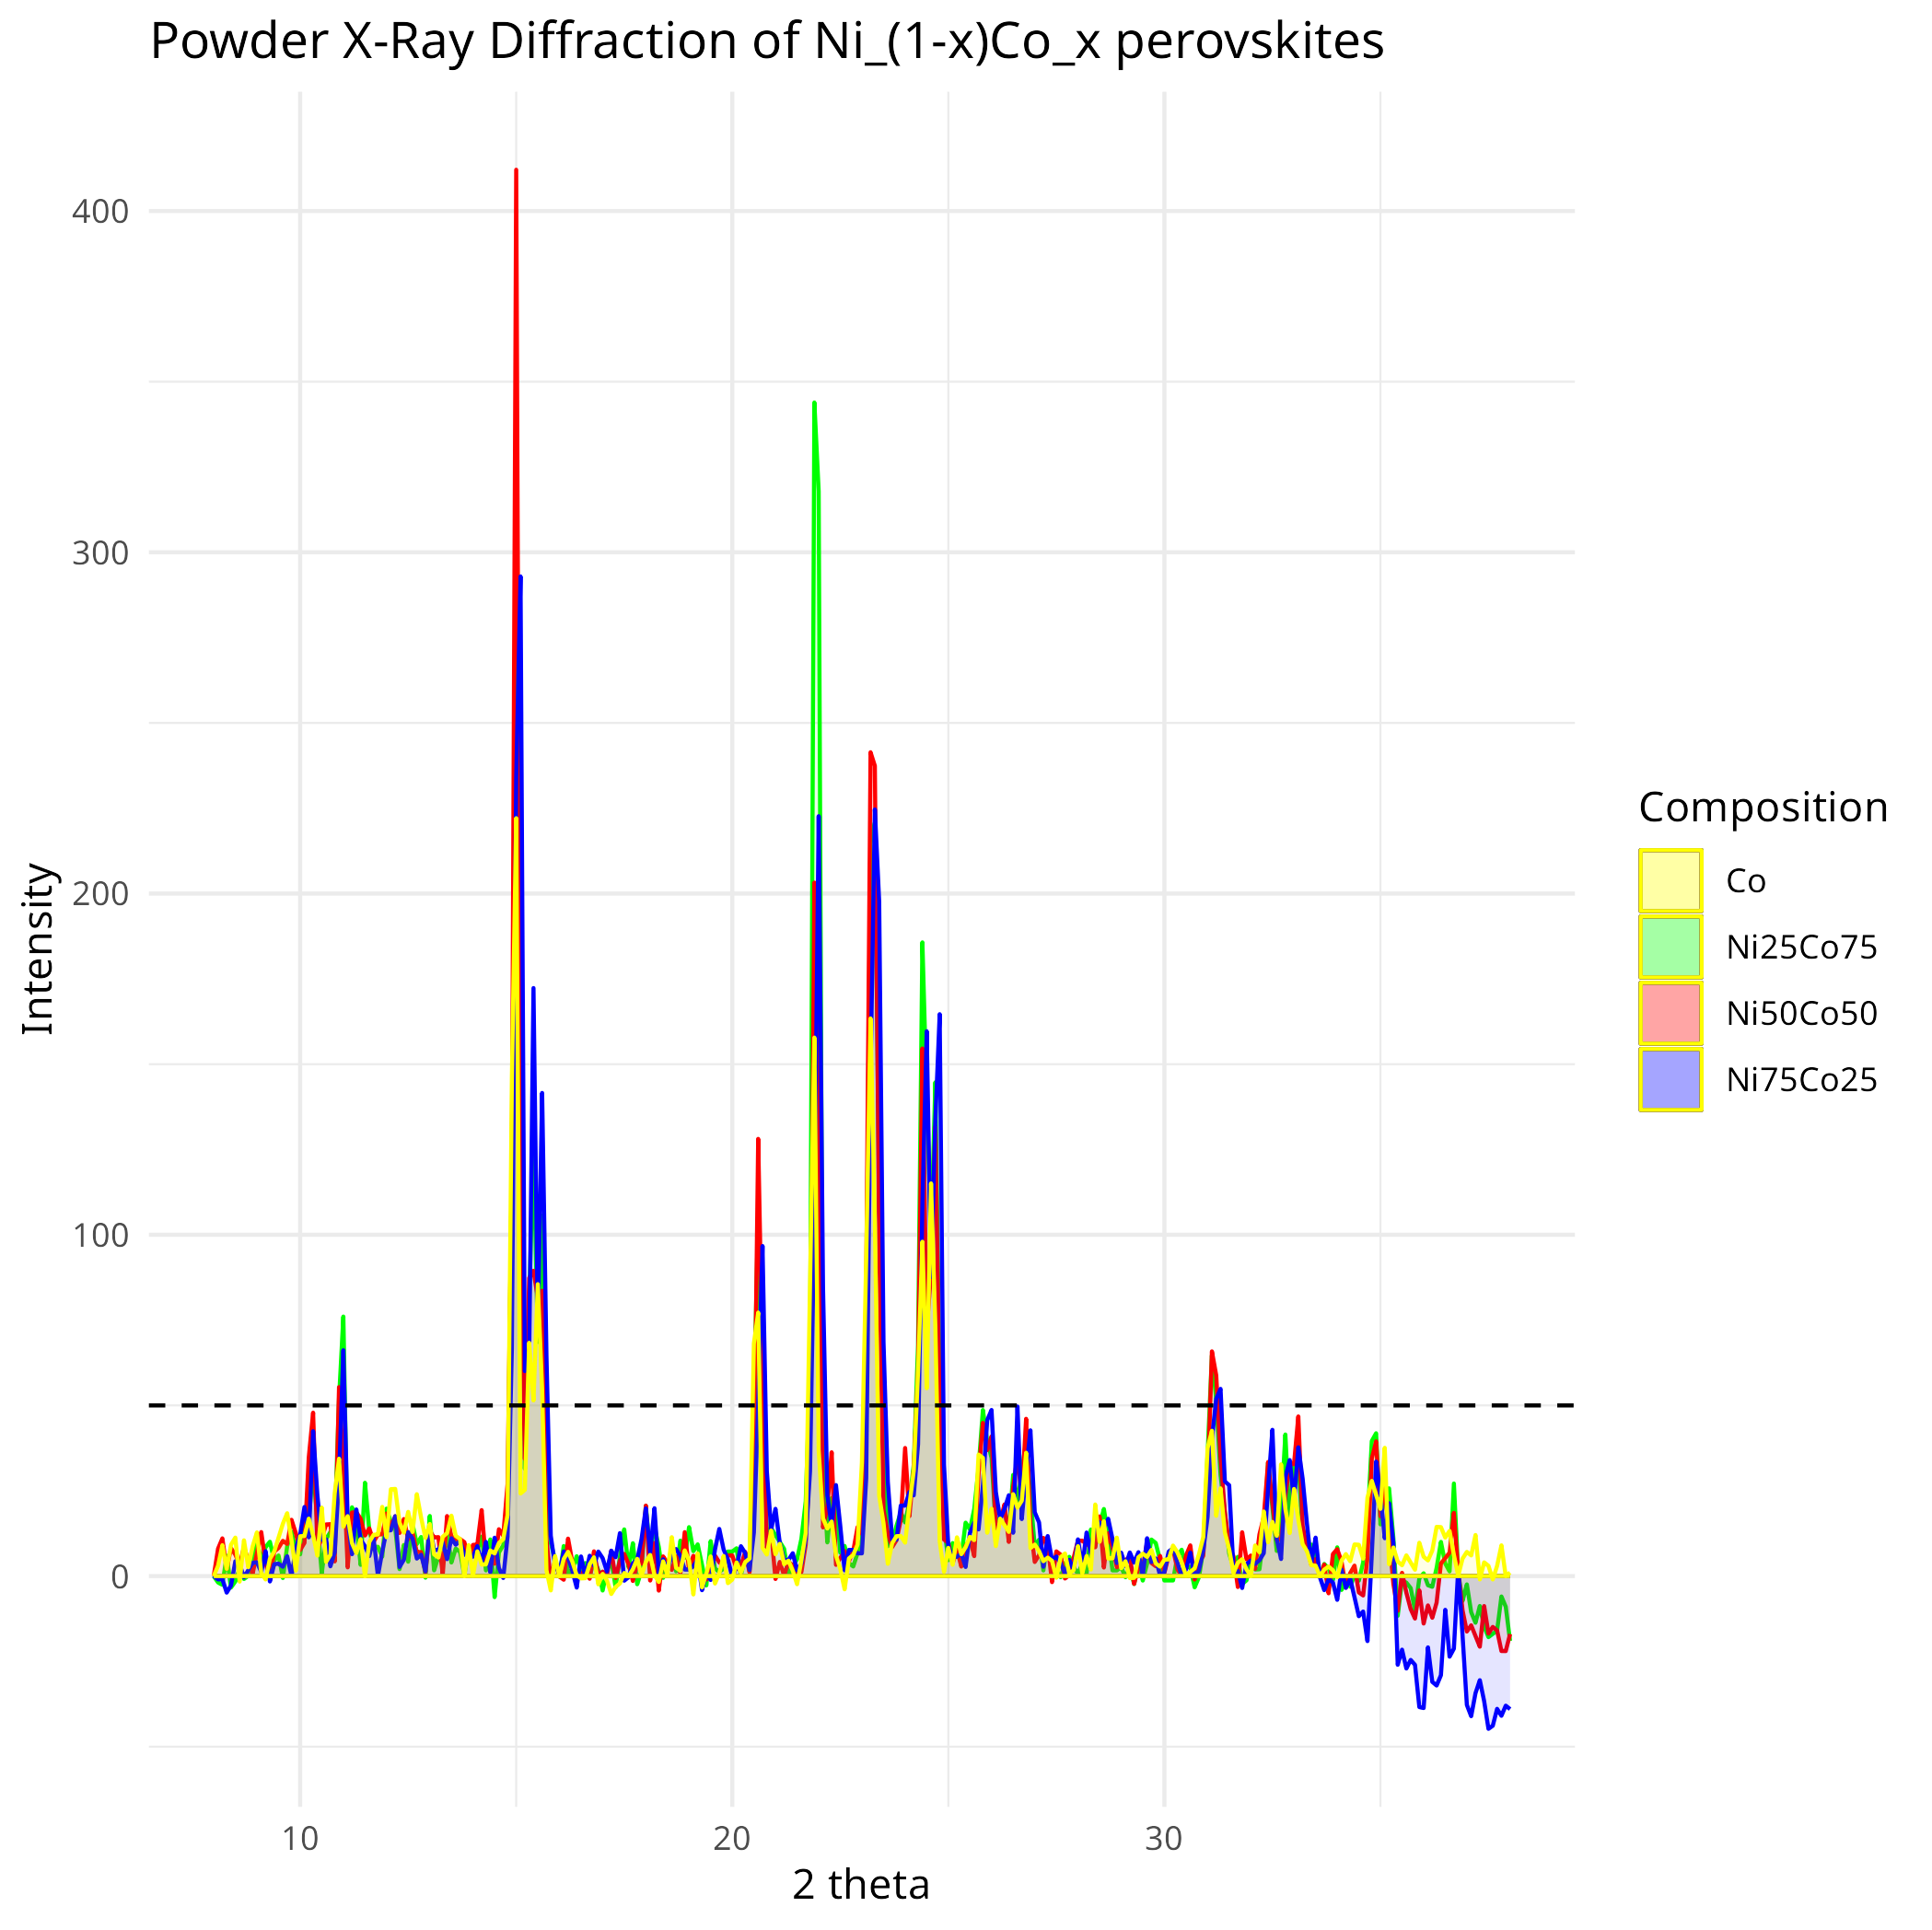
\includegraphics[width=0.8\textwidth]{../plot/graph.png}
        \caption{Powder X-ray Diffraction of Ni\_(1-x)Co\_x perovskites}
        \label{fig:xrd}
    \end{figure}
\end{frame}

\begin{frame}[fragile]{ANOVA Testing}
    \begin{itemize}
        \item Analysis of Variance (ANOVA) to test hypotheses.
        \item Results and interpretation.
    \end{itemize}

    \begin{lstlisting}[language=R]
    # ANOVA Testing
    anova_result <- aov(`2_theta` ~ Condition * Cluster, data = data_long)
    summary(anova_result)
    \end{lstlisting}
\end{frame}

\begin{frame}{Results and Discussion}
    \begin{itemize}
        \item Interpretation of ANOVA results.
        \item Comparison of clusters: Assessing the significance of peak position variations.
        \item Implications of the findings: Understanding how composition affects peak positions.
    \end{itemize}
\end{frame}

\begin{frame}{Conclusion}
    \begin{itemize}
        \item Summary of key findings.
        \item Limitations and areas for future research.
    \end{itemize}
\end{frame}

\begin{frame}{Questions \& Discussion}
    \centering
    \Huge Any Questions?
\end{frame}

\end{document}

